\documentclass[12pt,a4paper]{article}
\usepackage[utf8]{inputenc}

\usepackage{amsmath}
\usepackage{amsfonts}
\usepackage{amssymb}
\usepackage{graphicx}
\usepackage{listings}
\usepackage[margin=1.0in]{geometry}
\usepackage{caption}
\usepackage{subcaption}
\usepackage{float}
\usepackage[utf8]{inputenc}
\usepackage{refstyle}
\usepackage{spverbatim}
\usepackage{listings}
\usepackage{csvsimple}
\usepackage{adjustbox}
\usepackage{cancel}
\usepackage{scalerel,stackengine}
\stackMath
\newcommand\reallywidehat[1]{%
\savestack{\tmpbox}{\stretchto{%
  \scaleto{%
    \scalerel*[\widthof{\ensuremath{#1}}]{\kern-.6pt\bigwedge\kern-.6pt}%
    {\rule[-\textheight/2]{1ex}{\textheight}}%WIDTH-LIMITED BIG WEDGE
  }{\textheight}% 
}{0.5ex}}%
\stackon[1pt]{#1}{\tmpbox}%
}
\parskip 1ex

\lstset{numbers=left,
	title=\lstname,
	numberstyle=\tiny, 
	breaklines=true,
	tabsize=4,
	language=Python,
	morekeywords={with,super,as},,
	frame=single,
	basicstyle=\footnotesize\tt,
	commentstyle=\color{comment},
	keywordstyle=\color{keyword},
	stringstyle=\color{string},
	backgroundcolor=\color{background},
	showstringspaces=false,
	numbers=left,
	numbersep=5pt,
	literate=
		{æ}{{\ae}}1
		{å}{{\aa}}1
		{ø}{{\o}}1
		{Æ}{{\AE}}1
		{Å}{{\AA}}1
		{Ø}{{\O}}1
	}

\usepackage{bm}
\usepackage{hyperref}
\usepackage[usenames, dvipsnames]{color}

\begin{document}

\begin{center}
\LARGE{\textbf{Project 1}}
\\
\large{\textbf{Course: FYS-STK4155}}
\\
\large{\textbf{Semester: Autumn 2020}}
\\
\large{\textbf{Name: Sander Losnedahl}}
\end{center}


\newpage

\begin{center}
\Large{\textbf{Exercise 1.}}
\end{center}

\noindent \textbf{a)} The goal for this part of the exercise is trying to fit a linear model (linear in terms of regression coefficients) to the Franke function given as

\begin{equation}\label{eq:Franke}
\begin{aligned}
f(x,y) &= \frac{3}{4}\exp{\left(-\frac{(9x-2)^2}{4} - \frac{(9y-2)^2}{4}\right)}+\frac{3}{4}\exp{\left(-\frac{(9x+1)^2}{49}- \frac{(9y+1)}{10}\right)} \\
&+\frac{1}{2}\exp{\left(-\frac{(9x-7)^2}{4} - \frac{(9y-3)^2}{4}\right)} -\frac{1}{5}\exp{\left(-(9x-4)^2 - (9y-7)^2\right) }
\end{aligned}
\end{equation}

\noindent where polynomial combinations of x and y in the span $x,y \in [0,1]$ will be the explanatory variables. The linear regression equation then takes the form

\begin{equation}\label{eq:LinReg}
\begin{aligned}
\reallywidehat{f(x,y)} = \hat{y} = \textbf{X} \boldsymbol{\beta + \epsilon}
\end{aligned}
\end{equation}

\noindent where $\reallywidehat{f(x,y)}$ or $\hat{y}$ is the least squares estimate of the Franke function, $\textbf{X}$ is the $n\times p$ design matrix consisting of the aforementioned polynomial combinations of x and y, $\boldsymbol{\beta}$ are the $p\times 1$ regression coefficients and $\boldsymbol{\epsilon}$ is just random noise/unobserved random variables. In order to get the best estimate for the Franke function, we want to choose $\boldsymbol{\beta}$-values so that we minimize the residual sum of squares (thereby the name "least squares"). Solving equation \ref{eq:LinReg} with the intent to minimize the residual sum of squares yields the estimates for the $\boldsymbol{\beta}$-values 

\begin{equation}\label{eq:minBeta}
\begin{aligned}
\hat{\boldsymbol{\beta}} = (\textbf{X}^T\textbf{X})^{-1}\textbf{X}^T f(x,y)
\end{aligned}
\end{equation}

\noindent where T marks the transpose of the matrix. We can now get the estimate $\hat{\boldsymbol{\beta}}$ with equation \ref{eq:minBeta} and then compute the estimate of the Franke function as seen in equation \ref{eq:LinReg}. There is always uncertainty when estimating $\hat{\boldsymbol{\beta}}$. These uncertainties can be quantified by finding the confidence interval ($95\%$ confidence intervals in this case) around each coefficient. The interval will then be given by $\pm$ the standard deviation of the respective coefficients. In other words, we can be $95\%$ sure that the true coefficient will lie in the span of $[\beta_i - \sigma,\beta_i, \beta_i + \sigma]$. We can investigate this further by plotting each coefficient calculated from the ordinary least squares (equation \ref{eq:minBeta}) with their respective confidence intervals as seen in figure \ref{fig:polydegree}

\begin{figure}[H]
\centering
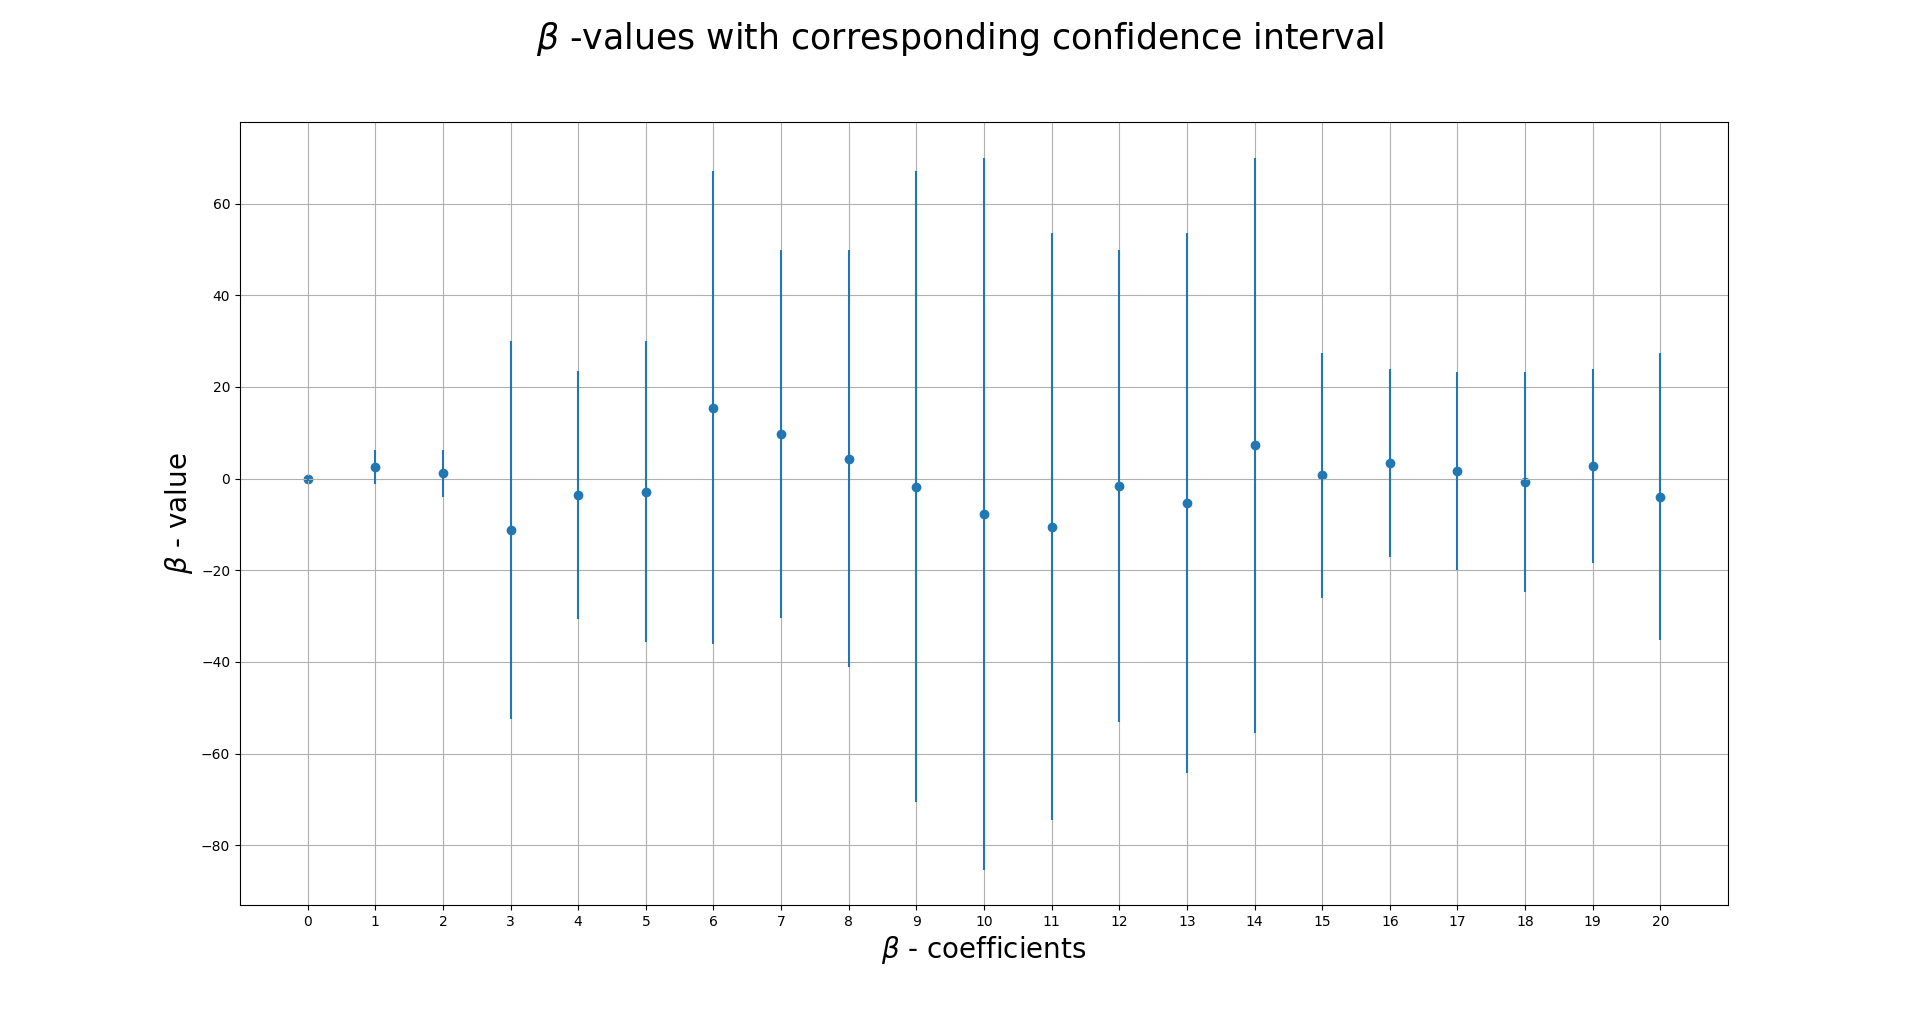
\includegraphics[width = 1\textwidth]{C:/Users/Sander/Documents/GitHub/FYS-STK4155/Project1/Report/Figures/1a2.PNG}
\caption{\label{fig:polydegree} $\hat{\boldsymbol{\beta}}$-coefficients from performing ordinary least squares regression Dots indicate the actual $\hat{\boldsymbol{\beta}}$-coefficients value while bars around indicate the $95\%$ confidence interval ($\pm \sigma$).}
\end{figure}

From figure \ref{fig:polydegree}, it can be observed that some coefficients have relatively narrow confidence intervals, while others have relatively large. The larger the interval, the less certain we are of the actual estimate. 

\newpage

\noindent \textbf{b)} When we fit a linear mode like in equation \ref{eq:LinReg}, we always want to minimize the mean square error (MSE). The MSE is often a good reference of the performance of our model and where lower MSE indicates a better model, and vice versa. The MSE is simply the expected value of the difference between the actual response and the predicted response using regression, which in math term is written as $E[(y-\hat{y})^2]$ where y is the actual response while $\hat{y}$ is the predicted response (as we already know). By adding and subtracting the term $E[\hat{y}]$ to the innter bracket we can expand the MSE like in equation qqqqqq

\begin{equation}\label{eq:mseDerive}
\begin{aligned}
MSE = E[(y-\hat{y})^2] = E[(y-\hat{y} + E[\hat{y}] - E[\hat{y}])^2]
\\
E[(\hat{y} - E[\hat{y}])^2 + 2(\hat{y} - E[\hat{y}])(E[\hat{y}]-y) + (E[\hat{y}]-y)^2]
\\
E[(\hat{y} - E[\hat{y}])^2] + E[2(\hat{y} - E[\hat{y}])(E[\hat{y}]-y)] + E[(E[\hat{y}]-y)^2]
\end{aligned}
\end{equation}

\noindent Since the expected value of $\hat{y}$ equals y, we can write $E[\hat{y}] - y =$ constant and thus

\begin{equation}\label{eq:mseDerive2}
\begin{aligned}
E[(\hat{y} - E[\hat{y}])^2] + 2(E[\hat{y}]-y)E[\hat{y}-E[\hat{y}]] + (E[\hat{y}]-y)^2
\\
E[(\hat{y} - E[\hat{y}])^2] + 2(E[\hat{y}]-y)(E[\hat{y}] - E[\hat{y}])+ (E[\hat{y}]-y)^2
\\
E[(\hat{y} - E[\hat{y}])^2] + (E[\hat{y}]-y)^2
\end{aligned}
\end{equation}

where the constant $E[\hat{y}] - E[\hat{y}]$ equals zero, making the whole term equal zero. 
\\
We recognize the term $E[(\hat{y} - E[\hat{y}])^2]$ as the variance of estimator $\hat{y}$ and the term $(E[\hat{y}]-y)^2$ as the difference between the bias, but squared. The bias quantifies how well the model fits the data points and variance is how well the model would translate to other data the model is not trained on. Increasing one tends to decrease the other, but not linearly since the bias is squared. Therefore, one can decrease the bias to a certain extent, but at some point, the loss of bias is not worth the gain in variance. This is called the bias variance trade-off. We can analyse the bias variance trade-off by plotting the MSE for different polynomial degrees (complexity of model) versus their respective MSE-values

\begin{figure}[H]
\centering
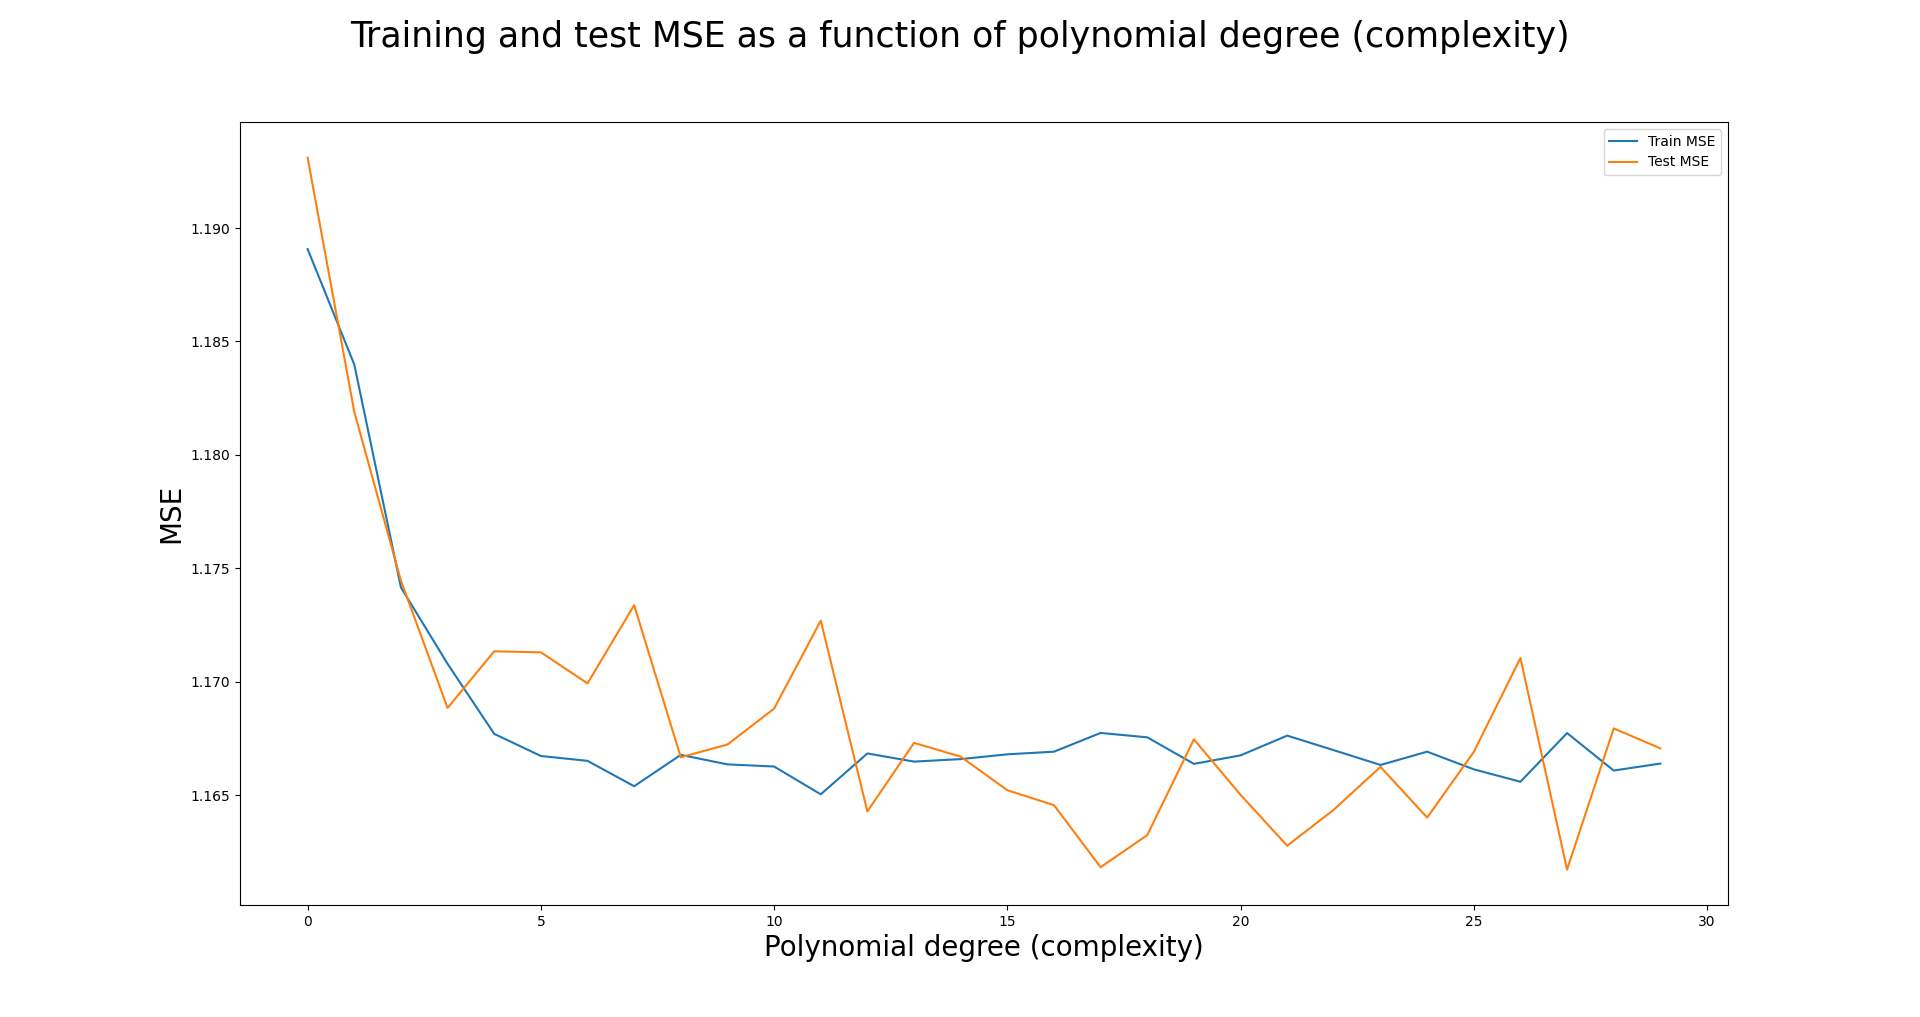
\includegraphics[width = 1\textwidth]{C:/Users/Sander/Documents/GitHub/FYS-STK4155/Project1/Report/Figures/polyVSMSEn1000p30.PNG}
\caption{\label{fig:bvto} MSE (variance + $\textrm{bias}^2$ as a function of polynomial degree (complexity of model).}
\end{figure}

\newpage

\begin{center}
\Large{\textbf{References}}
\end{center}

\begin{itemize}
  \item Reference
\end{itemize}

\end{document}
